\documentclass[tikz,border=0pt]{standalone}
\usepackage[T1]{fontenc}
\usepackage[sfdefault]{FiraSans}
\usepackage{tikz}
\usetikzlibrary{arrows.meta,positioning,calc,decorations.pathreplacing}
\definecolor{navy}{HTML}{003C6C}
\definecolor{navydeep}{HTML}{06294A}
\definecolor{ink}{HTML}{18293B}
\definecolor{muted}{HTML}{5B6B7C}
\definecolor{gold}{HTML}{FDC700}
\definecolor{amber}{HTML}{C98A00}
\definecolor{teal}{HTML}{0E7C9C}
\definecolor{coral}{HTML}{E4572E}
\definecolor{hairline}{HTML}{D9E1E9}
\definecolor{skyfill}{HTML}{E7F0F7}

\begin{document}
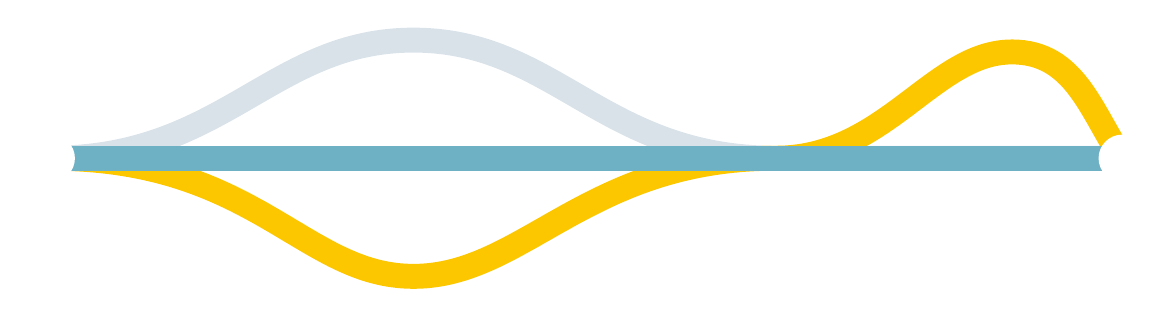
\begin{tikzpicture}

  \begin{scope}[line width=9pt, line cap=round]
    \draw[white!85!navy]  (0,0) .. controls (2.2,0) and (2.8,1.5) .. (4.6,1.5)
                          .. controls (6.4,1.5) and (7.0,0) .. (9.2,0)
                          .. controls (11.4,0) and (12.0,0) .. (13.6,0);
    \draw[gold]           (0,0) .. controls (2.6,0) and (3.2,-1.5) .. (4.6,-1.5)
                          .. controls (6.0,-1.5) and (6.8,0) .. (9.2,0)
                          .. controls (10.6,0) and (11.2,1.35) .. (12.2,1.35)
                          .. controls (13.0,1.35) and (13.2,0.6) .. (13.6,0);
    \draw[teal!60!white]  (0,0) -- (13.6,0);
    \fill[white] (0,0) circle (0.3) (13.6,0) circle (0.3);
  \end{scope}
\end{tikzpicture}
\end{document}
